%%%%%%%%%%%%%%%%%%%%%%%%%%%%%%%%%%%%%%%%%%%%%%%%%%%%%%%%%%%%%%%%%%%%%%
% writeLaTeX Example: A quick guide to LaTeX
%
% Source: Dave Richeson (divisbyzero.com), Dickinson College
%
% A one-size-fits-all LaTeX cheat sheet. Kept to two pages, so it
% can be printed (double-sided) on one piece of paper
%
% Feel free to distribute this example, but please keep the referral
% to divisbyzero.com
%
%%%%%%%%%%%%%%%%%%%%%%%%%%%%%%%%%%%%%%%%%%%%%%%%%%%%%%%%%%%%%%%%%%%%%%
% How to use writeLaTeX:
%
% You edit the source code here on the left, and the preview on the
% right shows you the result within a few seconds.
%
% Bookmark this page and share the URL with your co-authors. They can
% edit at the same time!
%
% You can upload figures, bibliographies, custom classes and
% styles using the files menu.
%
% If you're new to LaTeX, the wikibook is a great place to start:
% http://en.wikibooks.org/wiki/LaTeX
%
%%%%%%%%%%%%%%%%%%%%%%%%%%%%%%%%%%%%%%%%%%%%%%%%%%%%%%%%%%%%%%%%%%%%%%

\documentclass[10pt,landscape,letter]{article}
\usepackage{amssymb,amsmath,amsthm,amsfonts}
\usepackage{multicol,multirow}
\usepackage{calc}
\usepackage{ifthen}
\usepackage{graphicx}
\graphicspath{ {./} }

\usepackage[landscape]{geometry}
\usepackage[colorlinks=true,citecolor=blue,linkcolor=blue]{hyperref}
\usepackage{enumitem}
\usepackage[
bibbreaks=tight,
paragraphs=tight,
floats=tight,
mathspacing=tight,
wordspacing=tight,
tracking=tight,
bibnotes=tight,
charwidths=tight,
mathdisplays=tight,
leading=tight,
indent=tight,
lists=tight,
bibliography=tight,
title=tight,
sections=tight,
margins=tight
]{savetrees}
\newlist{Description}{description}{1}
\setlist[Description]{labelindent=2\parindent,leftmargin=2\parindent}

\usepackage{listings}

\lstset{
   basicstyle=\scriptsize\ttfamily,
   keywordstyle=\color{blue},
   stringstyle=\ttfamily, % stringstyle=\color{green}\ttfamily,
   commentstyle=\ttfamily, % commentstyle=\color{gray}\ttfamily,
   emph={square},
   emphstyle=\color{blue}\texttt,
   emph={[2]root,base},
   emphstyle=\texttt, % emphstyle={\color{gray}\texttt},
   showstringspaces=false,
   flexiblecolumns=false,
   tabsize=1,
   upquote=true,
   numbers=left,
   numberstyle=\tiny,
   numberblanklines=false,
   stepnumber=1,
   numbersep=8pt,
   xleftmargin=5pt,
   frame=single,
   language=sh
}

\ifthenelse{\lengthtest { \paperwidth = 11in }}
    { \geometry{top=.5in,left=.5in,right=.5in,bottom=.5in} }
	{\ifthenelse{ \lengthtest{ \paperwidth = 297mm}}
		{\geometry{top=1cm,left=1cm,right=1cm,bottom=1cm} }
		{\geometry{top=1cm,left=1cm,right=1cm,bottom=1cm} }
	}
\pagestyle{empty}
\makeatletter
\renewcommand{\section}{\@startsection{section}{1}{0mm}%
                                {-1ex plus -.5ex minus -.2ex}%
                                {0.5ex plus .2ex}%x
                                {\normalfont\large\bfseries}}
\renewcommand{\subsection}{\@startsection{subsection}{2}{0mm}%
                                {-1explus -.5ex minus -.2ex}%
                                {0.5ex plus .2ex}%
                                {\normalfont\normalsize\bfseries}}
\renewcommand{\subsubsection}{\@startsection{subsubsection}{3}{0mm}%
                                {-1ex plus -.5ex minus -.2ex}%
                                {1ex plus .2ex}%
                                {\normalfont\small\bfseries}}
\makeatother
\setcounter{secnumdepth}{0}
\setlength{\parindent}{0pt}
\setlength{\parskip}{0pt plus 0.5ex}
% -----------------------------------------------------------------------

\title{OpenZFS Cheat Sheet}

\begin{document}

\raggedright
\footnotesize

\begin{center}
	\Large{\textbf{OpenZFS Cheat Sheet}}
\end{center}
\begin{multicols}{3}
	\setlength{\premulticols}{1pt}
	\setlength{\postmulticols}{1pt}
	\setlength{\multicolsep}{1pt}
	\setlength{\columnsep}{2pt}


  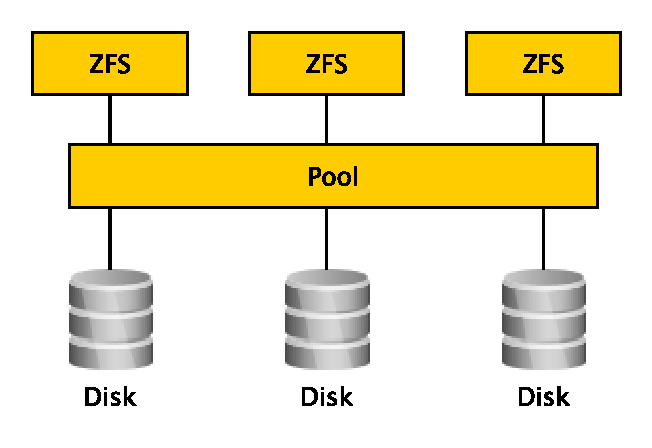
\includegraphics[width=0.3\textwidth]{archzfs}

	\section{Storage Pool Configurations}
  \begin{Description}%[leftmargin=0pt]
    \item[Single Disk] \textbf{Not redundant}, mounted as
      \texttt{/mypool}, there is no need for an entry in \texttt{/etc/fstab}.
      \texttt{zpool create mypool disk1}
    \item[Stripe (RAID-0)] \textbf{No redundancy, loss of all data if any one
      disk dies}. High performance, full disk space of all disks usable.\\
      \texttt{zpool create mystripe disk1	disk2}
    \item[Mirror (RAID-1)] Survives failure of one drive, VDEV shown as
      \texttt{mirror-0} in \texttt{zpool status} output, parallel reads of all
      disks, slow writes on all disks, lower total capacity compared to
      RAID-0.\\ \texttt{zpool create mymirror mirror disk1 disk2}
    \item[Single-Parity (RAID-Z1)] Requires at least 3 disks, survives one failing
      disk, parity information gets distributed across all disks, fast reads and
      writes with comparable performance, 66\% total capacity. Shown as
      \texttt{raidz1-0} VDEV in \texttt{zpool status} output.\\ \texttt{zpool create
      paritypool raidz disk1 disk2 disk3}
    \item[Double-Parity (RAID-Z2)] survives the failure of two disks per VDEV,
      slower than RAID-Z1, 4 disks required, 50\% capacity.
      \texttt{zpool create myraidz2 raidz2 disk1 disk2 disk3 disk4}
    \item[RAID10] Min.\ of 4 disks needed, survives failure of 2 disks (one per VDEV)
      high read speeds, write speed half of that, capacity 50\%. Good compromise
      between redundancy, capacity and performance.\\ \texttt{zpool create
      myr10 mirror disk1 disk2 mirror disk3 disk4}
    \item[Triple-Parity (RAID-Z3)] Little slower than RAID-Z2, redundancy of
      three disks per VDEV, min. 5 disks required, 40\% capacity.
      \texttt{zpool create myz3 raidz3 disk1 disk2 disk3 disk4 disk5}
  \end{Description}

	\section{Display Pool Status}
	\begin{Description}
    \item[\texttt{zpool status}] Display pool status including disk
      configuration, any errors and applicable updates, last scrub (if any).
		\item[\texttt{zpool list}] Show pool capacity, used and free space.
    \item[\texttt{zpool iostat}] Display pool I/O statistics. Options
      display individual devices (\texttt{-v}), I/O latency (\texttt{-w}),
      request size histograms (\texttt{-r}), wait (\texttt{-l}) and queue
      statistics (\texttt{-q}).
    \item[\texttt{zpool history}] Administrative command history of the pool.
      Options include long form (\texttt{-l}) or events like transaction groups
      (\texttt{-i}).
    \item[\texttt{zpool get}] Properties and values, change \texttt{default}s
      via \texttt{zpool set}.
	\end{Description}

  \section{Special VDEVs}
	\begin{Description}
    \item[Level 2 ARC (L2ARC)] A fast read cache for cases where data does not
      fit in the ZFS main memory cache (ARC: adaptive replacement cache)
      anymore. Reads will then served out of the L2ARC, which requires a fast
      storage device (flash) to see benefits. Use the \texttt{cache} keyword to
      add such a device to a pool. \texttt{zpool add mypool cache /dev/nda0}
    \item[ZFS Intent Log (ZIL)] Changes synchronous into asynchronous writes
      (does not affect reads). Applications get faster confirmation of written
      data and hence acts like a database transaction log. Gets cleared once
      the writes have reached the underlying pool storage media. Requires fast
      storage media, but does not need to be big. Use the \texttt{log} keyword
      to add to a pool: \texttt{zpool add mypool log /dev/nda1}
    \item[Spare] Does not take I/O until replaced (manually or by external
      failure management software) with a failed pool disk. Add to a pool with
      the \texttt{spare} keyword: \texttt{zpool add mypool spare /dev/nda2}
  \end{Description}

  \section{Pool Extension}
	\begin{Description}
    \item[Turn single disk pool into RAID1] The single disk pool device
      \texttt{nda0} gets the mirror partner disk \texttt{nda1} attached:
      \texttt{zpool attach mypool mirror /dev/nda0 /dev/nda1}
    \item[Replace failed disk] Exchange the failed pool disk \texttt{nda2} with
  device \texttt{nda3}: \texttt{zpool replace mypool /dev/nda2 /dev/nda3}
  \end{Description}

  \section{Pool Import/Export}
	\begin{Description}
    \item[Export] Finishes and closes I/O operations, then unmounts the pool
      from the filesystem hierarchy. Attach to a different system and import
      there to reconstruct the pool state. \texttt{zpool export mypool}

    \item[Import] Imports pools into the running system.
      \begin{itemize}
        \item Scan for ZFS pool signatures: \texttt{zpool import}
        \item Import a pool via ID or its name: \texttt{zpool import mypool}
        \item Renames a pool: \texttt{zpool import oldname newname}
        \item Mount the imported pool under a different path to prevent
          shadowing existing ones: \texttt{zpool import -R /media mypool}
        \item Import readonly: \texttt{zpool import -o readonly mypool}
        \item Try restoring recently destroyed pool: \texttt{zpool import -D mypool}
      \end{itemize}
	\end{Description}

	\section{ZFS Datasets}
  Datasets sit on top of the pool and consume its space. Addressed like this:
  \texttt{mypool/data}. Each pool creates a default dataset with its own
  name as top level.
  \textbf{Example:} \texttt{zpool create test disk1}\\ creates a pool and
  dataset called \texttt{test}, which may hold child datasets beneath. Mounts
  the top-level pool as the \texttt{/test} dataset.
	\begin{Description}
    \item[Create new dataset] Creates a new dataset called \texttt{ds},
      inherits most properties of the parent dataset: \texttt{zfs create
      mypool/ds}\\ Create multiple datasets: \texttt{zfs create -p mypool/home/fred}
      \item [Display datasets] List the used, available space, and mountpoint: \texttt{zfs list}
        \begin{itemize}
          \item Show dataset by ZFS path: \texttt{zfs list mypool/ds}
          \item List datasets and any children:
            \texttt{zfs list -r mypool/ds}
          \item Limit display depth of datasets:
            \texttt{zfs list -d 1 mypool/home}
          \item Display dataset name only:
            \texttt{zfs list -o name mypool/home}
          \item Remove output headers, too:
            \texttt{zfs list -Ho name mypool/home}
          \item Change display order:
            \texttt{zfs list -o used,avail,refer,name}
          \item Sort output by column:
            \texttt{zfs list -rs refer mypool/home}
          \item Reverse sort order:
            \texttt{zfs list -rS refer mypool/home}
        \end{itemize}
    \item[Display available pool space] Lists available and used space per
      dataset and children, including snapshots and any reservations:
      \texttt{zfs list -o space} \textbf{Recommendation:} use instead of
      \texttt{df -h}.
    \item[Rename dataset] Rename dataset or move to a different place within
      the pool hierarchy, comparable to the Unix \texttt{mv} command.\\
      \texttt{zfs rename mypool/home/fred mypool/home/eva}

    \item[Destroy dataset] Simulate first: \texttt{zfs destroy -nv mypool/old}\\
      \textbf{Output:} \texttt{would destroy mypool/old}\\
      Remove and show result: \texttt{zfs destroy -v
      mypool/old}\\ \textbf{Output:} \texttt{will destroy
      mypool/old}\\ Recursively destroy datasets:
      \texttt{zfs destroy -r mypool/testdata}
	\end{Description}

	\section{Properties}
  Dataset use is flexible by inheriting most of their parents properties. Children
  may override these if necessary. Change only \texttt{default} properties in the
  \texttt{SOURCE} column. The same goes for pool properties.
	\begin{Description}
    \item[Display properties] There are various ways to display properties:
      \begin{itemize}
        \item Show pool properties: \texttt{zpool get all mypool}
        \item Display all properties of a dataset: \texttt{zfs get all \texttt{pool/dataset}}
        \item List single property (\texttt{capacity}): \texttt{zpool get capacity mypool}
        \item List multiple properties: \texttt{zpool get capacity,health mypool}
      \end{itemize}
    \item[Change properties] Deactivate access time property: \texttt{zfs set atime=off mypool}
      Change mountpoint: \texttt{zfs set mountpoint=/media mypool/ds}

    \item[Custom Properties] Define custom dataset property as a
      \texttt{key=value pair}. Datasets inherit them, but can change their
      value.
      \begin{itemize}
        \item Creation: \texttt{zfs set warranty:expires=2048/04/20 mypool}
      \item List custom property: \texttt{zfs get warranty:expires mypool}
      \item Reset the value: \texttt{zfs inherit warranty:expires mypool}
      \item Remove property: \texttt{zfs inherit -r warranty:expires mypool}
      \end{itemize}
	\end{Description}

  \section{Scrub} ZFS stores checksums alongside the data and in the whole
  dataset hierarchy. Different factors like I/O errors, malformed drivers or
  defective RAM, broken cables, etc.\ cause the checksum calculation to not
  match anymore. Given enough redundancy at the pool level (VDEVs), ZFS finds
  these errors and corrects them (self healing). Run monthly \texttt{scrub}s on
  the pool to re-calculate the checksums. If they do not match, ZFS asks the
  redundant VDEV for it and corrects the data if they match. \texttt{zpool
  scrub mypool} The \texttt{zpool status} output displays the progress of the
  scrub operation and any errors that were found. There is no \texttt{fsck} in
  ZFS since it is unnecessary.

	\section{Volumes}
  ZFS Volumes uses contiguous pool space to export via iSCSI over the network. When
  formatting a volume with a non-ZFS filesystem, then this filesystem uses
  all underlying ZFS features automatically.
	\begin{Description}
    \item[Volume creation] Create a 10~GB ZFS volume:
      \texttt{zfs create -V 10G mypool/vol1}
    \item[Create sparse volume] An overprovisioned volume that does not
      use the reserved space right away, but fills it up over time.
      \texttt{zfs create -V 1P -s mypool/sparse1PBvol}
	\end{Description}



  \newpage

	\section{Quota}
  Each dataset may use up the entire disk space of the pool. Quotas restrict
  that to certain user defined amounts. Writes that run over the quota are
  strictly stopped by ZFS to enforce the quotas.

	\begin{Description}

    \item[Define Quota] Datasets do not have a quota by
      default. Set a quota for a specific dataset using \texttt{zfs set}:
      \texttt{zfs set quota=10G mypool/dataset}\\ A quota restricts the
      dataset and any children (existing and future ones). Datasets
      share the total quota amongst themselves. If a quota should  apply to the
      parent dataset alone, then use: \texttt{zfs set refquota=10G mypool/dataset} ZFS quotas
      may also restrict certain daemons or users in the system: \texttt{zfs set
      userquota@fred=10G mypool/home/fred} A group quota restricts a collection
      of users as a whole: \texttt{zfs set groupquota@projectX=100G mypool/projectX}

		\item[Display quotas] Query the quota property using \texttt{zfs get}:
      \begin{itemize}
        \item List quotas for a given dataset: \texttt{zfs get quota mypool/dataset}
        \item Same for the \texttt{refquota}: \texttt{zfs get refquota mypool/home/fred}
        \item Display a userquota: \texttt{zfs userspace mypool/home/fred}
        \item Show group quotas: \texttt{zfs groupspace mypool/projectX}
      \end{itemize}
    \item[Remove quota] Return dataset to having no quota applied (same for \texttt{refquota}):
      \texttt{zfs set quota=none mypool/home/fred}
	\end{Description}

	\section{Reservation}
  Reservations guarantee a certain amount of available disk space in the pool,
  regardless of how much other datasets use. This reduces the total pool space
  for the reservation. This prevents any one dataset to use up the whole pool
  space and allows capacity planning.

	\begin{Description}
    \item[Define reservation] The \texttt{reservation} property controls the
      amount of disk space to reserve for a dataset: \texttt{zfs set
      reservation=100G mypool/home} Reservations apply to child datasets,
      too. Set the reservation to the dataset alone: \texttt{zfs set
      refreservation=10G mypool/home/eve}
    \item[Display reservation] Use the \texttt{reservation} property to show
      the dataset reservation: \texttt{zfs get reservation
      mypool/home/eve} Likewise, \texttt{zfs list -o space} shows the used
      reservation in the \texttt{USEDREFRESERV} column.
    \item[Remove reservation] Set \texttt{reservation} or
      \texttt{refreservation} to \texttt{none}: \texttt{zfs set
      reservation=none mypool/home/eve}
	\end{Description}

	\section{Snapshots}
  Snapshots provide a quick way of preserving a readonly state of the dataset
  at a certain time. Roll back a snapshot to return the dataset to the
  snapshot's creation time. Restoring individual files from the snapshot is
  also possible without a complete rollback. A hidden \texttt{.zfs} directory
  allows readonly access to individual files for this purpose.
	\begin{Description}
    \item[Snapshot creation] \texttt{zfs snapshot mypool/ds@mysnapshot}
      Short form: \texttt{zfs snap mypool/ds@mysnapshot}\\
      Recursive snapshot: \texttt{zfs snap -r mypool/ds@mysnapshot}
    \item[Display snapshots] List all dataset snapshots:
      \texttt{zfs list -t snap mypool/ds}\\
      List snapshots with all children:
      \texttt{zfs list -rt snap mypool/ds}
    \item[Show writes since last snapshot] The \texttt{written} property shows
      the amount of data written to the dataset since taking the last snapshot.
      In combination with \texttt{used} and \texttt{referenced} it gives a good
      overview of the necessary pool space: \texttt{zfs list -rt all -o
      name,used,refer,written mypool}
    \item[Compare snapshots] Use \texttt{zfs diff} to compare changes in the
      dataset since a particular snapshot:
		      \texttt{zfs diff mypool/ds@backup}\\
		      The table below describes the output:
		      \begin{center}
			      \begin{tabular}{ c | l }
				      \textbf{Character} & \textbf{Description} \\
				      \hline
				      $+$              & File added\\
				      $-$              & File deleted \\
				      M                & File modified\\
				      R                & File renamed \\
			      \end{tabular}
		      \end{center}
          Applied to directories means changes in the metadata. Compare two
          snapshots:
          \texttt{zfs diff mypool/ds@backup1 mypool/ds@backup2}
    \item[Snapshot rollback] Throws away the current dataset state and returns to
      the last snapshot state. Removes all created data since that particular snapshot.
      \texttt{zfs rollback mypool/ds@backup2}\\
      Rolling back to an earlier snapshot requires the removal of all intermediary snapshots:
      \texttt{zfs rollback -r mypool/ds@backup1}
    \item[Snapshot mounting] Mount a snapshot into the filesystem as a readonly dataset:
      \texttt{mount -t zfs mypool/ds@backup /mnt/backup}
    \item[Delete snapshot range] Execute a verbose (\texttt{-v}) dry run (\texttt{-n}) first to see
      what would get deleted:
      \texttt{zfs destroy -vn mypool/ds@backup}
      If this is the desired action, remove the dry run parameter \texttt{-n} to
      execute: \texttt{zfs destroy -v mypool/ds@backup} Recursively delete snapshots using \texttt{-r}: \texttt{zfs destroy -rv mypool/ds@backup}\\
    \item[Delete range] For snapshots \verb|@a| - \verb|@e|, define different ranges for deletion:
	\begin{itemize}
    \item Delete \verb|@b| through \verb|@d| (inclusive): \texttt{zfs destroy -v mypool@b\%d}
    \item Delete starting from snapshot \verb|@b|: \texttt{zfs destroy -v mypool@b\%}
    \item Delete snapshots before \verb|@b|: \verb|zfs destroy -v mypool@%b|
	\end{itemize}
\item[ZFS Holds] Preserve a snapshot by creating a hold referenced by a custom
  tag (description). ZFS allows multiple tags and only if the last tag is gone,
      the snapshot may be removed.
	\begin{itemize}
    \item Create new hold: \texttt{zfs hold keepme mypool/home@important}
    \item List holds recursively: \texttt{zfs holds -r mypool/home@important}
    \item Lift a hold again by tag: \texttt{zfs release mypool/home@important}
	\end{itemize}
	\end{Description}

	\section{Clones}
  A clone represents a writeable version of a snapshot. All the data from the
  snapshot they are based on are present in the clone, too.
	\begin{Description}
    \item[Clone creation] Create a clone from an existing snapshot using \texttt{zfs clone}:
      \texttt{zfs clone mypool/ds@backup mypool/myclone}
      The \texttt{origin} property of a clone contains the originating snapshot for reference: \texttt{zfs get origin mypool/myclone}
    \item[Make clone independent] ZFS prevents removing a snapshot as long as
      dependent clones still exist. Resolve this by reversing the dependency of clone and
      snapshot by promoting a clone to a full dataset: \texttt{zfs promote mypool/myclone}
      The \texttt{origin} property disappears and the snapshot is associated with the clone now.
    \item[Clone removal] Delete clones like regular datasets: \texttt{zfs destroy mypool/myclone}
	\end{Description}

  \section{Encryption}
  ZFS allows encrypting datasets with individual keys. Some metadata remains unencrypted to allow scrub and other operations to run.
	\begin{Description}
    \item[Create encrypted dataset] Set dataset encryption passphrase: \texttt{zfs create -o encryption=on -o keyformat=passphrase -o keylocation=prompt mypool/secret}
    \item[Load status] Get status: \texttt{zfs get keystatus mypool/secret}
    \item[Load key] Unencrypt dataset: \texttt{zfs load-key mypool/secret}
	\end{Description}


  \section{Delegation}
  ZFS allows delegating ZFS commands to non-root users.
	\begin{Description}
    \item[Delegate permission to user] Grant user the \texttt{atime} property
      permission on dataset: \texttt{zfs allow -u joe atime mypool/dataset}
    \item[Display delegations] Show existing dataset delegations: \texttt{zfs allow mypool/dataset}
    \item[Remove delegation] Use \texttt{zfs unallow} to remove \texttt{compression} permission:
      \texttt{zfs unallow -u joe compression mypool/dataset}
    \item[Delegate permission to group] Target a group:
      \texttt{zfs allow -g mygroup atime mypool/dataset}
    \item[Delegate permission to delegate] ZFS permits delegating those permissions that the delegating
      user possesses: \texttt{zfs allow -u jill allow
      mypool/dataset}
    \item[Create a set of permissions] A permission set allows combining multiple delegations under a user-defined name:
      \texttt{zfs allow -s @myset mount,snapshot,rollback,destroy mypool/dataset}
    \item[Use permission set for delegations] Apply permission set
      to grant permissions: \texttt{zfs allow -u jill @myset
      mypool/dataset}
	\end{Description}


	\section{Sending and Receiving Snapshots}
  ZFS allows transferring snapshots as a byte stream locally or over the
  network to the same or a different pool for backup purposes.
	\begin{Description}
    \item[Write snapshot to a file] Write a byte stream representation of the data to a file:
      \texttt{zfs send mypool/ds@backup > dsbackup}\\
      Restore this file to the same or a different
      pool using \texttt{zfs receive}. Display more details about the
      transfer using the \texttt{-v} parameter:\\
      \texttt{zfs send -v mypool/ds@backup > target}
    \item[Create dataset from snapshot] Use \texttt{receive} (or: \texttt{recv}) to re-create dataset from snapshot:
      \texttt{zfs recv mypool/backup < dsbackup}
      Display transfer details using the \texttt{-v} parameter: \texttt{zfs recv -v
      mypool/backup < dsbackup}
    \item[Replication without intermediary file] A pipe between \texttt{zfs
      send} and \texttt{zfs recv} combines the input and output: \texttt{zfs send
      mypool/ds@backup|zfs recv mypool/new}
    \item[Replication via SSH] Send snapshots over SSH to another pool on a different host:
      \texttt{zfs send poolA/ds@backup|ssh host zfs recv poolB/new}\\
    \item[Send permissions] Allow non-root user \texttt{sender} to send
      datasets: \texttt{zfs allow -u sender send,snapshot mypool/source}
    \item[Receive permissions] Non-root user \texttt{receiver} requires more
      permissions: \texttt{zfs allow -u receiver
      compression,mountpoint,mount,create,receive mypool/destination}
  \end{Description}


	\vfill

	\hrule
	% ~\\
	Benedict Reuschling (\texttt{benedict@reuschling.org}), April~2025
	\newpage

\end{multicols}
\end{document}
